\documentclass[11pt,aspectratio=169]{beamer}

\usepackage[utf8]{inputenc}
\usepackage[T1]{fontenc}
\usepackage[french]{babel}
\usepackage{amsmath,amssymb}
\usepackage{xcolor}
\usepackage{booktabs}
\usepackage{array}
\usepackage{tabularx}
\usepackage{graphicx}
\usepackage{tikz}
\usetikzlibrary{positioning,arrows.meta,backgrounds,fit}

% ---------- Couleurs ----------
\definecolor{navy}{HTML}{1B2F4E}
\definecolor{accent}{HTML}{2E5FA3}
\definecolor{softgray}{HTML}{F4F6FA}
\definecolor{cream}{HTML}{FFF9F0}

% ---------- Thème ----------
\usetheme{Madrid}
\usecolortheme{default}
\setbeamercolor{structure}{fg=accent}
\setbeamercolor{title}{fg=white,bg=navy}
\setbeamercolor{frametitle}{fg=white,bg=navy}
\setbeamercolor{palette primary}{fg=white,bg=navy}
\setbeamercolor{palette secondary}{fg=white,bg=accent}
\setbeamercolor{palette tertiary}{fg=white,bg=navy}
\setbeamercolor{block title}{fg=white,bg=accent}
\setbeamercolor{block body}{fg=black,bg=softgray}
\setbeamertemplate{navigation symbols}{}
\setbeamertemplate{itemize items}[circle]

\title[Maquette $\to$ Modèle]{De la maquette au modèle}
\subtitle{Notre cas d'étude, expliqué pas à pas}
\author{Note de synthèse --- Recherche Master II}
\date{\today}

\begin{document}

% ============================================================
\begin{frame}
\titlepage
\end{frame}

\begin{frame}{Plan}
\tableofcontents
\end{frame}

% ============================================================
\section{Notre cas d'étude}
% ============================================================

\begin{frame}{Le cas d'étude que nous allons suivre}
\begin{columns}[T]
\begin{column}{0.42\textwidth}
\centering
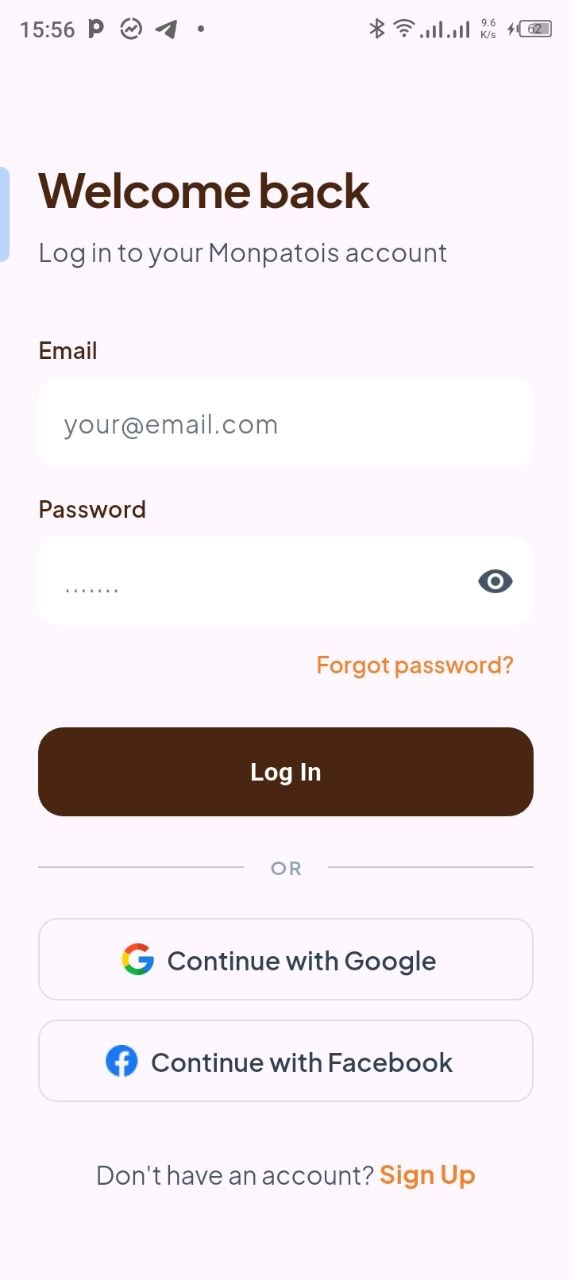
\includegraphics[height=0.75\textheight]{maquette.jpg}
\end{column}
\begin{column}{0.58\textwidth}



\vspace{0.4cm}
\begin{block}{Objectif final}
Comprendre comment cette image se transforme en un \textbf{modèle structuré} (graphe puis arbre), avant génération de code.
\end{block}
\end{column}
\end{columns}
\end{frame}

% ============================================================
\section{La maquette haute fidélité}
% ============================================================

\begin{frame}{Qu'est-ce qu'une maquette haute fidélité ?}
\begin{columns}[T]
\begin{column}{0.35\textwidth}
\centering
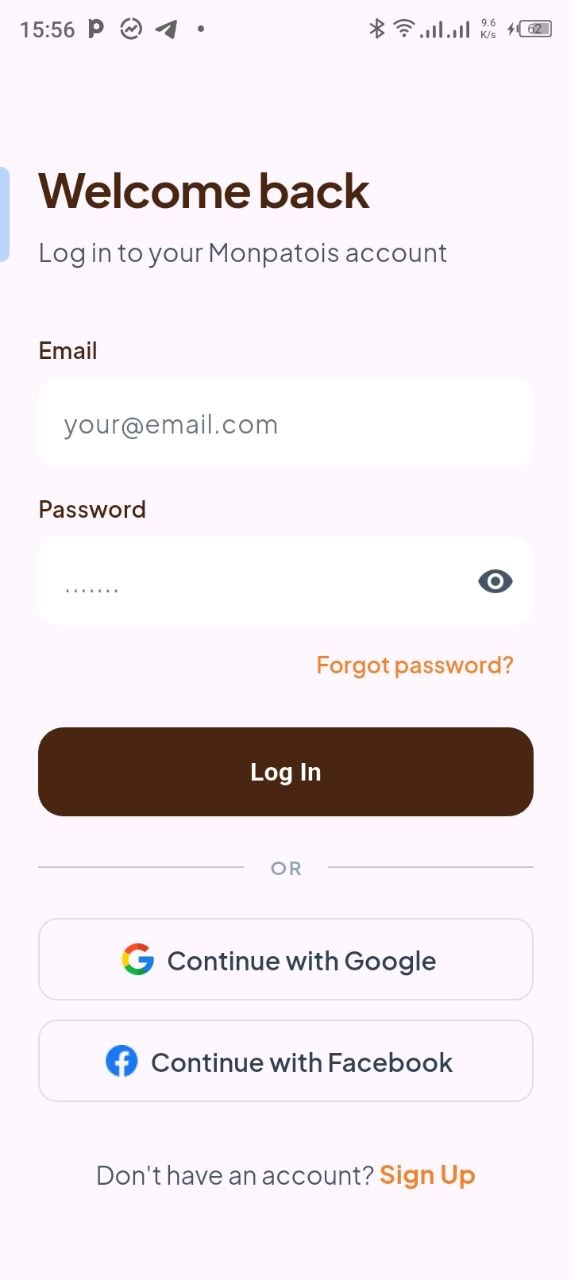
\includegraphics[height=0.75\textheight]{maquette.jpg}
\end{column}
\begin{column}{0.65\textwidth}
Ce que vous voyez à gauche \textbf{est} une maquette haute fidélité (\emph{high-fidelity mockup}) : une représentation qui reproduit fidèlement ce que verra l'utilisateur final mêmes couleurs, mêmes polices, mêmes espacements
, mêmes textes.
ils est differents des maquettes basse fidélité (\emph{low-fidelity mockups}) qui sont plus schématiques, avec des blocs gris et du texte générique (\emph{lorem ipsum}). et permet ainsi de se concentrer sur la structure et le contenu plutôt que sur l'apparence exacte.

\vspace{0.4cm}

\end{column}
\end{columns}
\end{frame}



\begin{frame}{Caractéristiques principales --- pointées sur notre maquette}
\centering
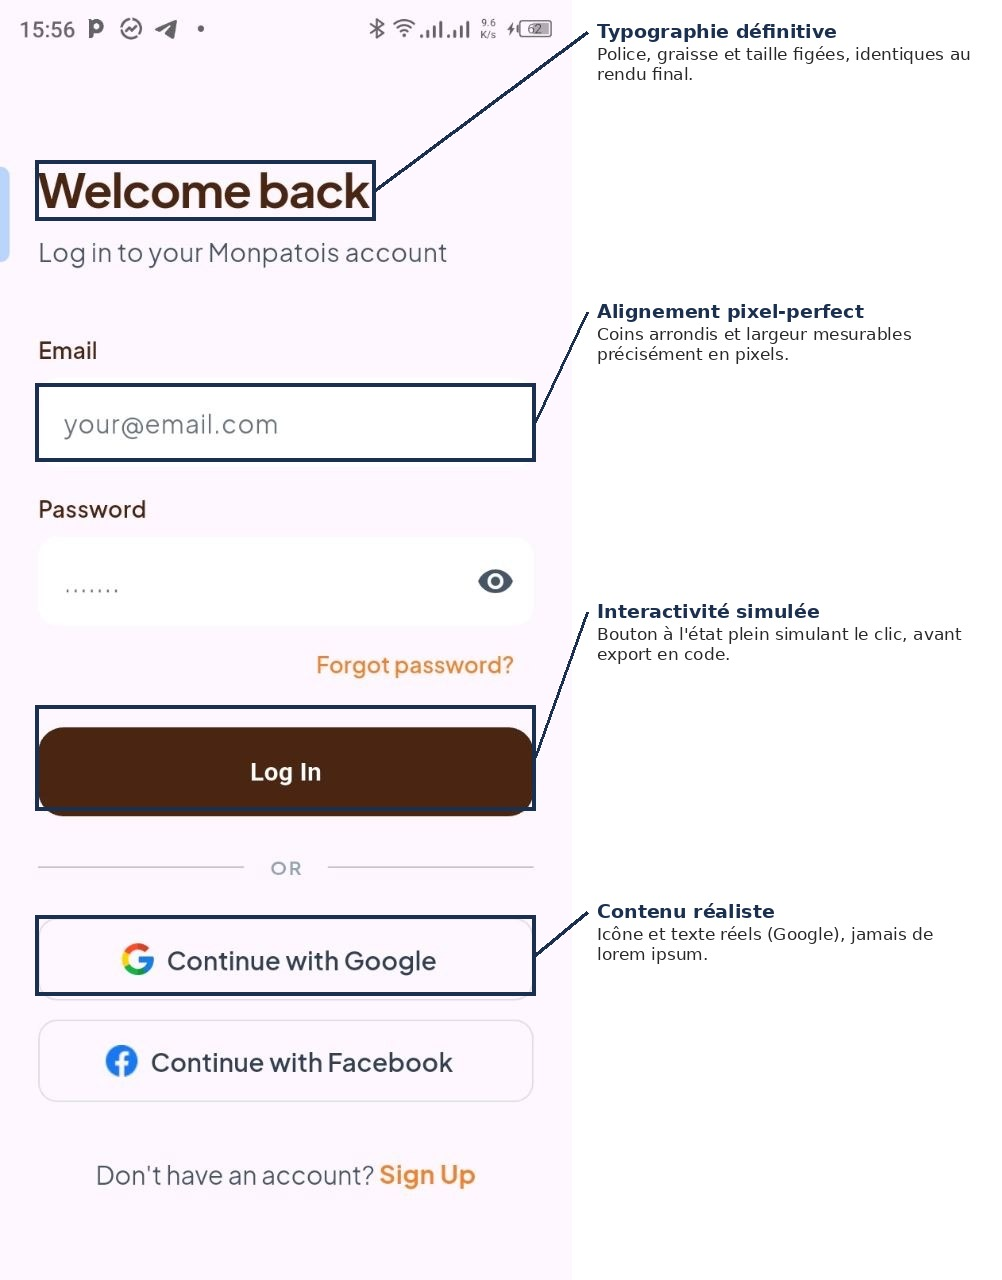
\includegraphics[height=0.85\textheight]{maquette_characteristics.jpg}
\end{frame}

\begin{frame}{Caractéristiques principales --- synthèse}
\small
\begin{tabularx}{\textwidth}{@{}lX@{}}
\toprule
\textbf{Caractéristique} & \textbf{Ce qu'on observe sur notre maquette} \\
\midrule
Précision visuelle & Couleurs exactes du bouton \emph{Log In}, typographie définitive du titre \\
Contenu réaliste & « your@email.com », icône Google réelle : pas de \emph{lorem ipsum} \\
Espacements cohérents & Marges verticales régulières entre label et champ \\
Interactivité simulée & Bouton \emph{Log In} à l'état plein, icône « œil » sur le mot de passe \\
Alignement pixel-perfect & Chaque champ a une position et une largeur mesurables en pixels \\
\bottomrule
\end{tabularx}
\end{frame}

\begin{frame}{Les éléments métriques --- de la maquette dans son ensemble}
\centering
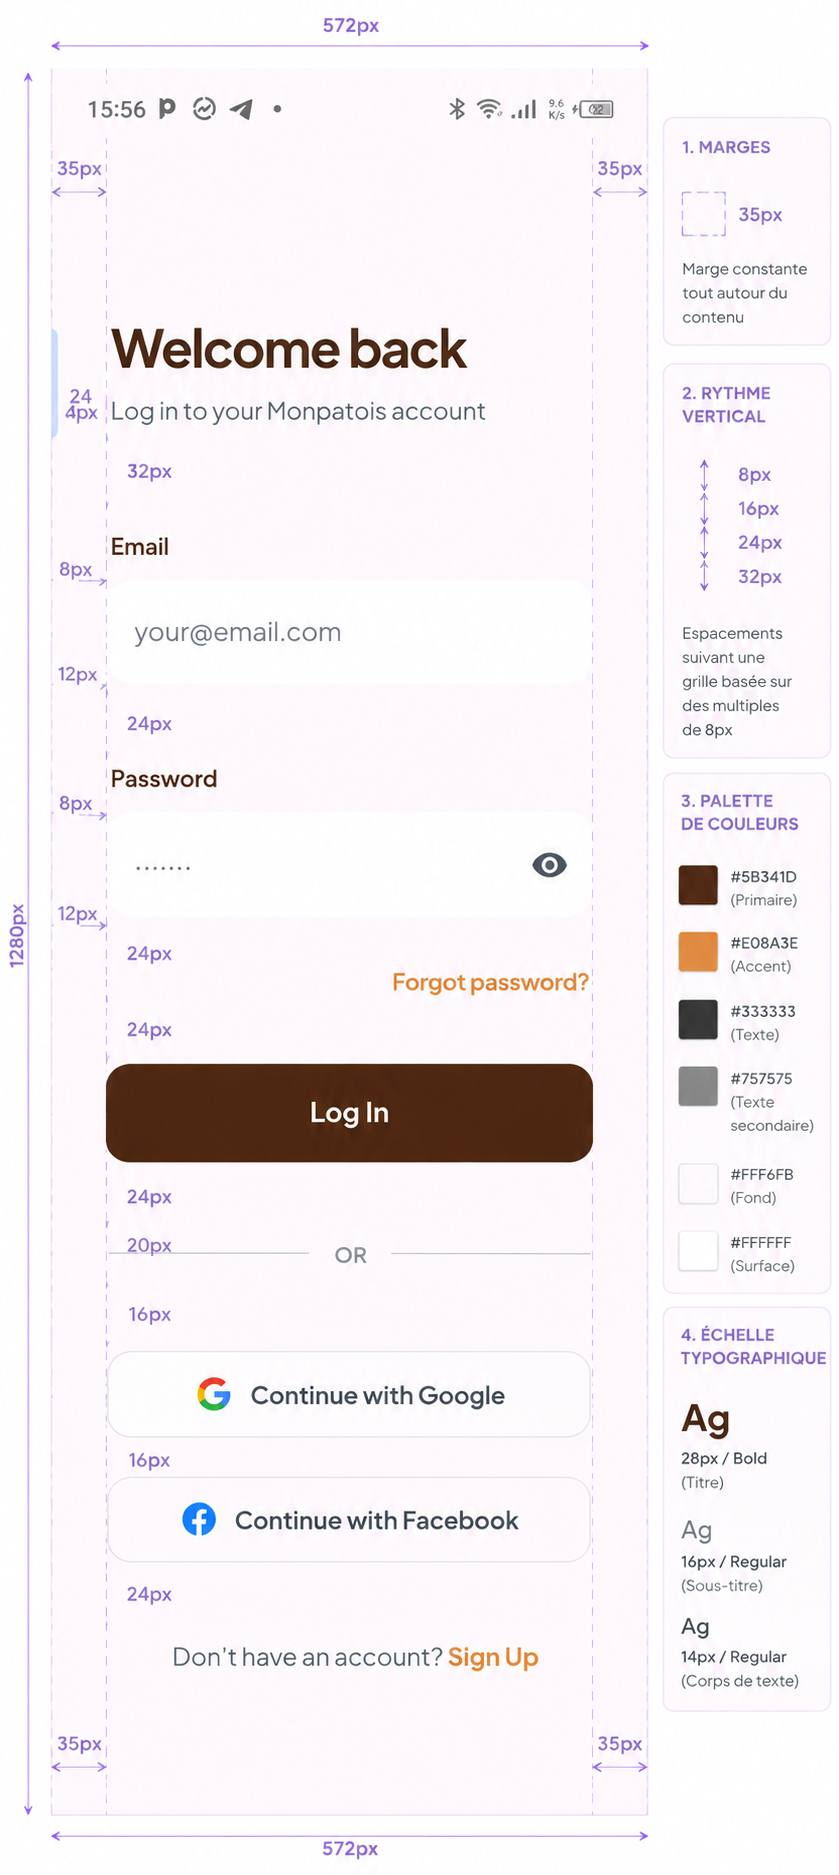
\includegraphics[height=0.85\textheight]{elements_metrics.jpg}
\end{frame}

\begin{frame}{Les éléments métriques --- synthèse}
Ce qu'on peut mesurer sur \textbf{la maquette entière}, pas seulement sur un élément isolé :
\begin{itemize}
    \item \textbf{Dimension du canevas} : $572 \times 1280$ px (taille totale de l'écran)
    \item \textbf{Marges} : distance constante entre le bord de l'écran et le contenu (ici $\approx$ 35 px de chaque côté)
    \item \textbf{Rythme vertical} : les espacements entre blocs successifs suivent une grille régulière ($\approx$ 20--30 px, multiples de 8 px)
    \item \textbf{Palette de couleurs} : un jeu limité de teintes réutilisées (fond, texte, bouton, accent)
    \item \textbf{Échelle typographique} : quelques tailles de police seulement (titre, sous-titre, corps de texte)
\end{itemize}

\vspace{0.3cm}
\begin{block}{Pourquoi c'est important}
Ces régularités (grille, palette, échelle) sont ce qui permettra plus tard de \textbf{déduire des règles de style génériques} lors de la génération de code, plutôt que de coder chaque pixel un par un.
\end{block}
\end{frame}

% ============================================================
\section{Le modèle}
% ============================================================

\begin{frame}{Qu'est-ce qu'un modèle ?}
Ici, \textbf{modèle} ne désigne pas un modèle d'IA, mais une \textbf{représentation structurée et abstraite} de la maquette que nous venons de voir, sous forme de graphe ou d'arbre.

\vspace{0.3cm}
Le modèle ne contient plus de pixels : il contient
\begin{itemize}
    \item des \textbf{éléments} (les 18 composants de notre écran de connexion)
    \item des \textbf{relations} entre eux (proximité, appartenance, hiérarchie)
\end{itemize}

\vspace{0.3cm}
\begin{block}{Analogie}
La maquette est une photo de famille ; le modèle est l'arbre généalogique.\\
La photo montre les visages, l'arbre montre qui est le parent de qui.
\end{block}
\end{frame}
\begin{frame}{-- representation}
\centering
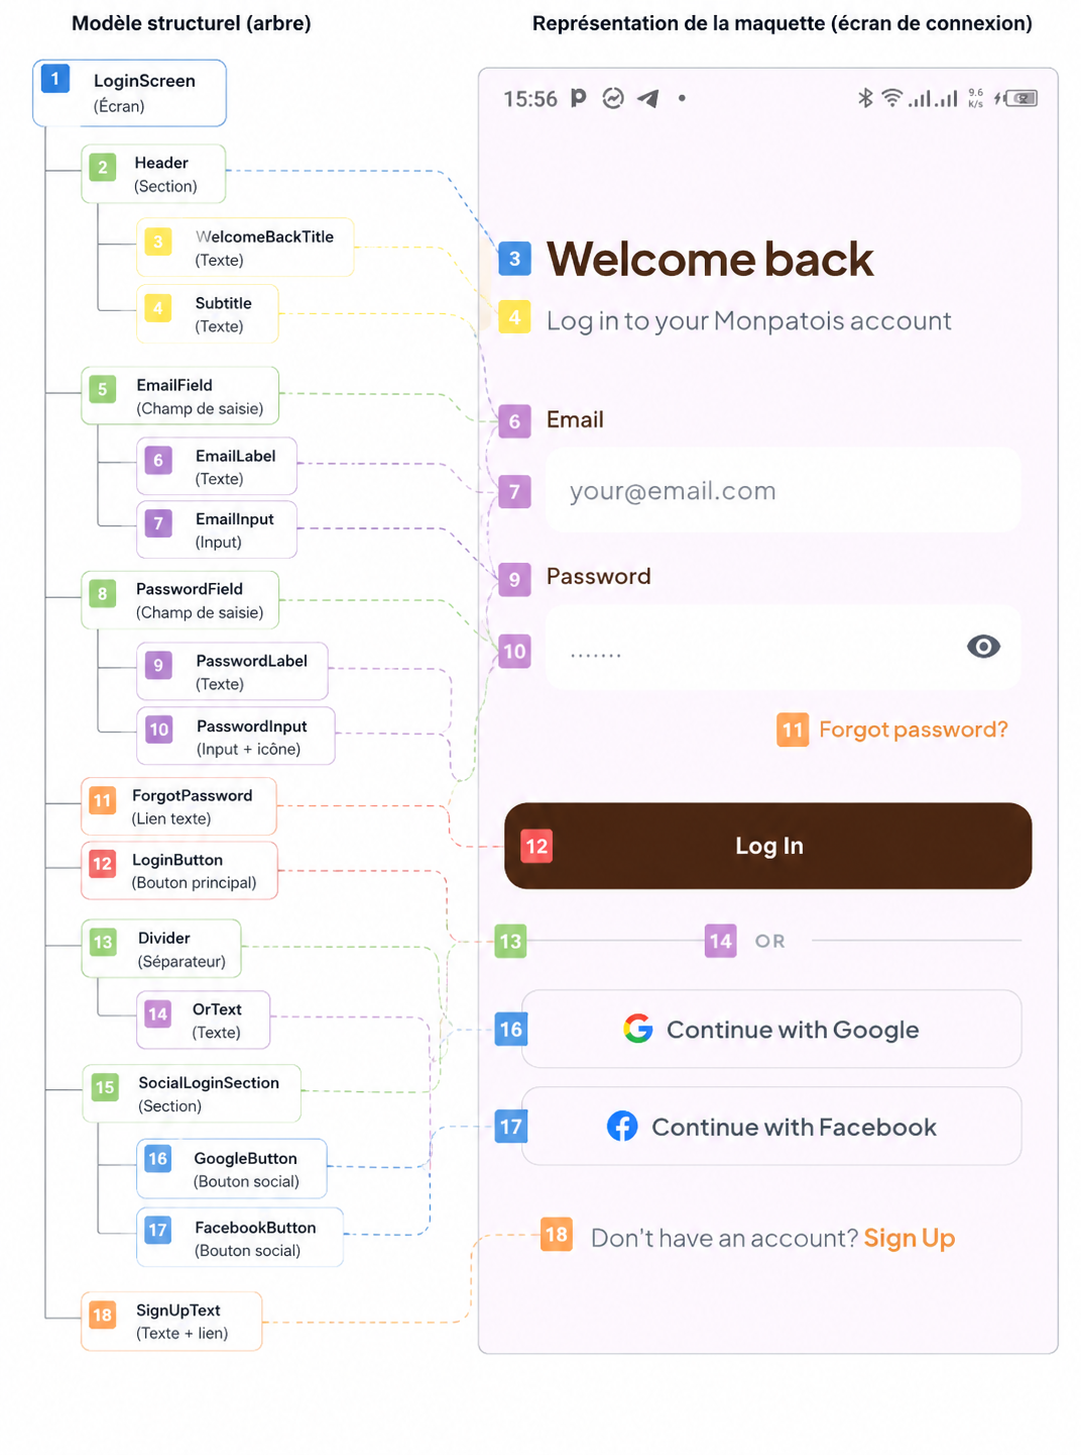
\includegraphics[height=0.85\textheight]{element_maquette.png}
\end{frame}

\begin{frame}{Les deux formes du modèle}
\begin{enumerate}
    \item \textbf{Le graphe de relations}\\
    Chaque élément de notre maquette devient un n\oe{}ud. Deux n\oe{}uds reliés s'ils sont proches ou similaires.\\
    $\to$ répond à : \emph{« quels éléments vont ensemble ? »}
    \vspace{0.3cm}
    \item \textbf{L'arbre de layout}\\
    Les groupes obtenus s'organisent en hiérarchie (conteneurs, sous-conteneurs, éléments atomiques).\\
    $\to$ répond à : \emph{« comment ces groupes s'emboîtent-ils ? »}
\end{enumerate}
\end{frame}

\begin{frame}{-- representation}
\centering
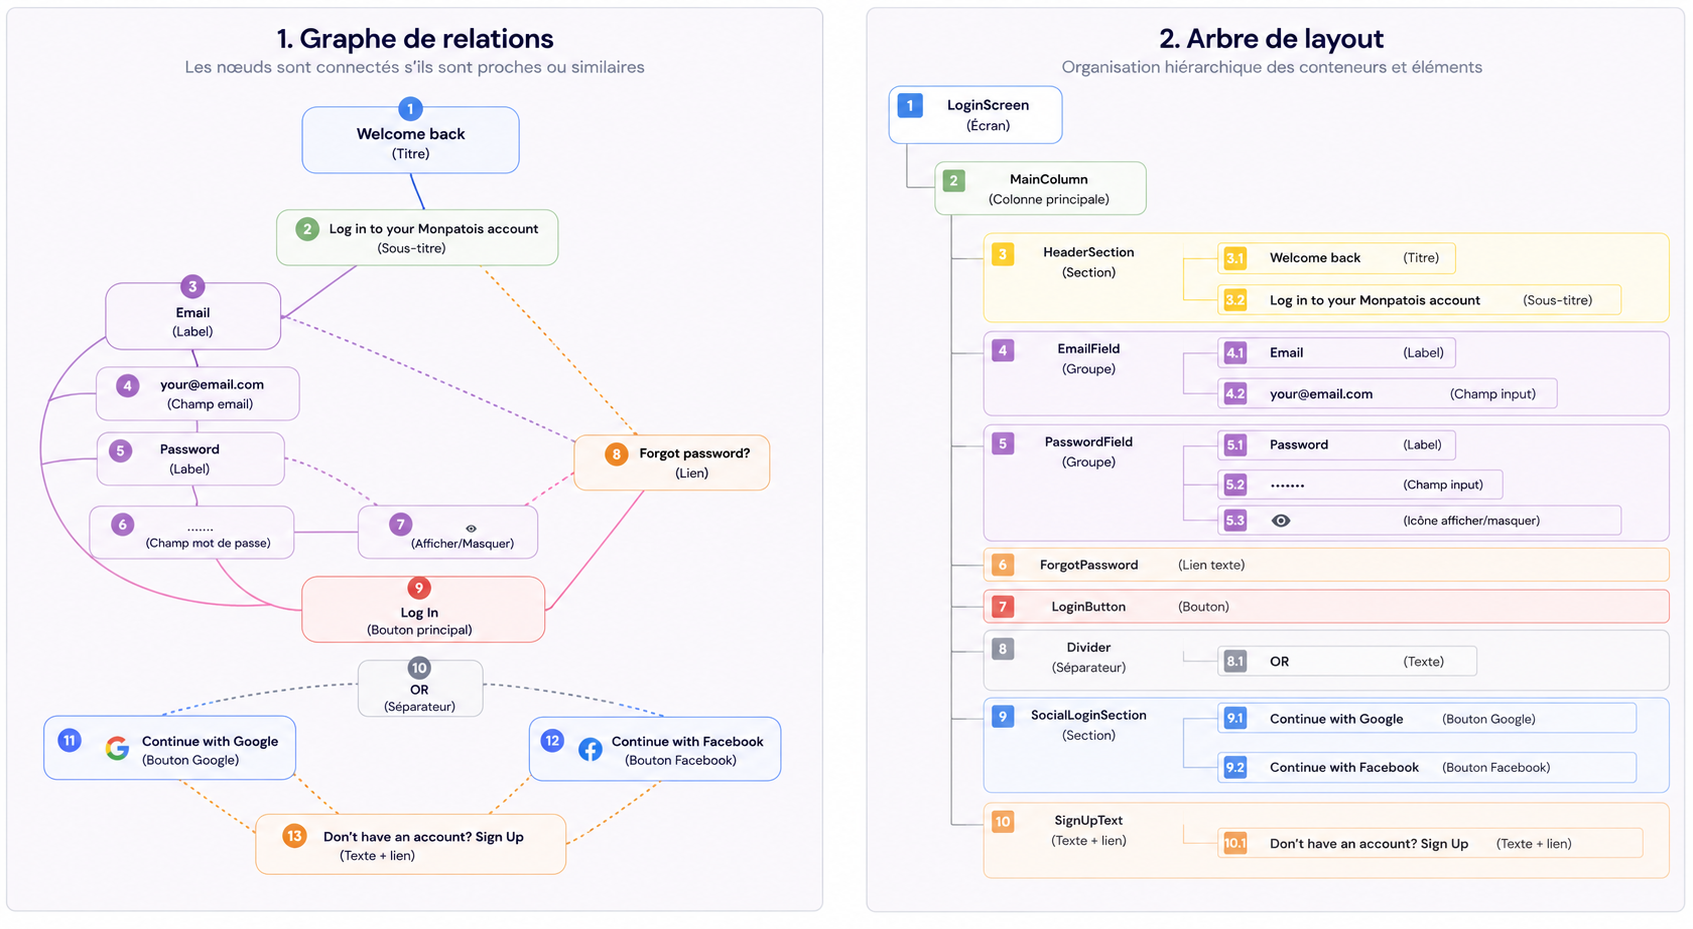
\includegraphics[height=0.85\textheight]{graphes.png}
\end{frame}

% ============================================================
\section{Détection sur notre maquette}
% ============================================================

\begin{frame}{Étape 1 --- Détection des boîtes sur notre maquette}

\centering
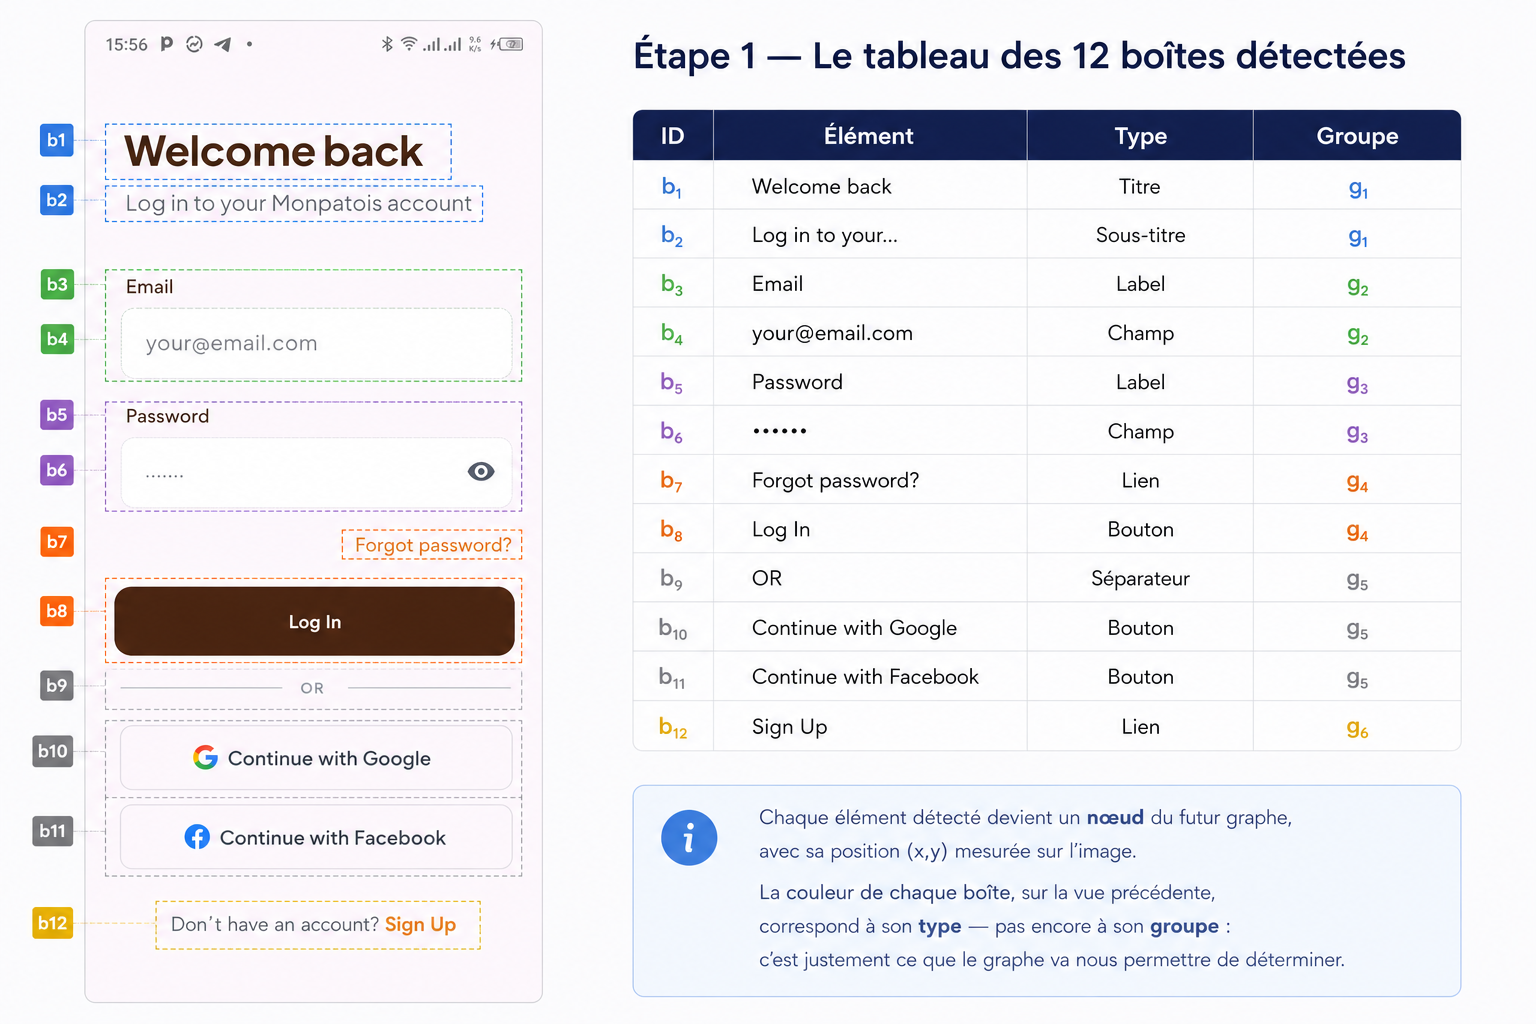
\includegraphics[height=0.85\textheight]{tableau_groupe.png}
\end{frame}


\begin{frame}{Comment décide-t-on qu'un lien existe ?}
Pour construire le graphe, on ne relie pas les éléments au hasard : on calcule un \textbf{score de similarité} $\sigma$ pour \emph{chaque paire} d'éléments détectés sur notre maquette.

\vspace{0.3cm}
\[
\sigma(b_i, b_j) = \alpha \cdot \text{sim}_{\text{geo}}(b_i,b_j) + \beta \cdot \text{sim}_{\text{sem}}(b_i,b_j)
\]
avec $\alpha + \beta = 1$

\vspace{0.3cm}
\begin{block}{Deux critères combinés}
\begin{itemize}
    \item $\text{sim}_{\text{geo}}$ : sont-ils \textbf{proches sur l'écran} ?
    \item $\text{sim}_{\text{sem}}$ : se \textbf{ressemblent-ils visuellement} (même style, même type) ?
\end{itemize}
\end{block}

Le score $\sigma$ est donc un compromis entre \emph{position} et \emph{apparence}.
\end{frame}

\begin{frame}{Attention : similarite geometrique et similarite sémantique sont deux choses différentes}
\begin{block}{À ne pas confondre}
\begin{itemize}
    \item $\text{sim}_{\text{geo}}$ mesure une \textbf{distance sur l'écran} (en pixels).
    \item $\text{sim}_{\text{sem}}$ mesure une \textbf{ressemblance visuelle} (couleur, forme, type d'élément) --- \emph{indépendamment} de la position.
\end{itemize}
Deux éléments peuvent être proches sans se ressembler, ou se ressembler sans être proches.
\end{block}
\end{frame}

\begin{frame}{similarite Geometrique}
\centering
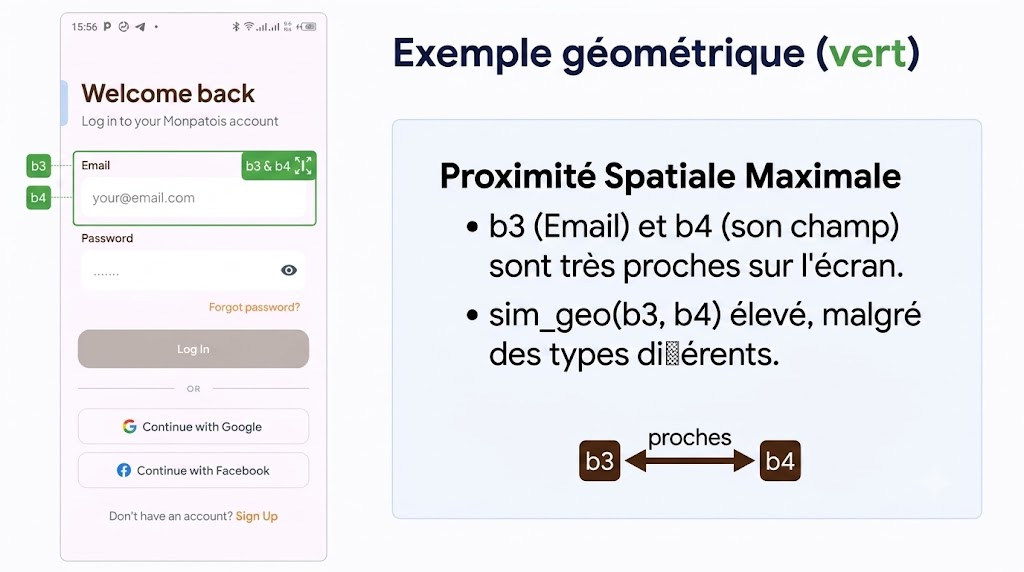
\includegraphics[height=0.85\textheight]{similarite_geometrique.jpg}
\end{frame}
\begin{frame}{similarite Semantique}
\centering
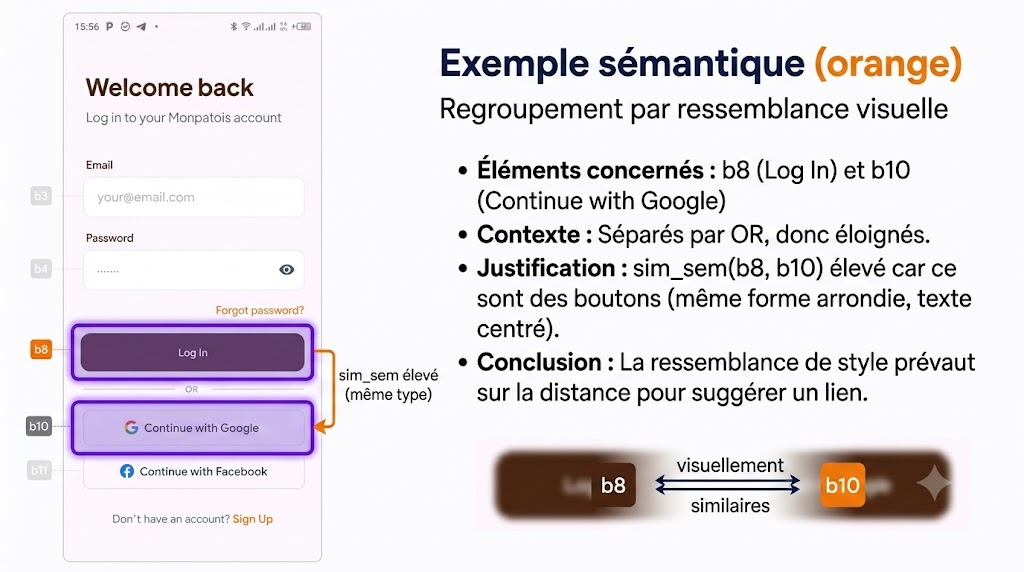
\includegraphics[height=0.85\textheight]{similarite_semantique.jpg}
\end{frame}

\begin{frame}{Le détail des deux calculs}
\textbf{1. Similarité géométrique} --- distance entre les coordonnées $(x,y)$ des deux boîtes (ex. $b_3$ et $b_4$ vus à l'instant), transformée en score entre 0 et 1 :
\[
\text{sim}_{\text{geo}}(b_i,b_j) = e^{-\,\text{distance}(b_i,b_j)/\tau}
\]
Plus la distance est petite, plus le score se rapproche de 1. $\tau$ règle la sensibilité à la distance.

\vspace{0.4cm}
\textbf{2. Similarité sémantique} --- chaque élément est résumé par un vecteur de caractéristiques visuelles $\phi(b_i)$ (couleur, forme, texte ou non). On compare deux vecteurs par cosinus :
\[
\text{sim}_{\text{sem}}(b_i,b_j) = \cos\big(\phi(b_i),\phi(b_j)\big)
\]
Deux éléments de même nature (les boutons $b_8$ et $b_{10}$ vus à l'instant, par exemple) obtiennent un score proche de 1, \textbf{même si} leur $\text{sim}_{\text{geo}}$ est plus faible.
\end{frame}

\begin{frame}{Lien fort ou lien faible : le rôle du seuil $\theta$}
Une fois $\sigma$ calculé pour une paire, on compare ce score à un \textbf{seuil} $\theta$ fixé à l'avance (ex. $\theta = 0{,}5$) :

\vspace{0.3cm}
\begin{block}{Règle de décision}
\[
\sigma(b_i,b_j) \geq \theta \;\Rightarrow\; \textbf{lien fort} \text{ (arête tracée)}
\]
\[
\sigma(b_i,b_j) < \theta \;\Rightarrow\; \textbf{lien faible} \text{ (pas d'arête)}
\]
\end{block}

\vspace{0.3cm}
Sur notre maquette : $b_3$ et $b_4$ franchissent le seuil, $b_3$ et $b_9$ non --- comme on l'a vu sur l'image précédente. Un « lien faible » ne se dessine pas : il correspond simplement à l'\textbf{absence} d'arête entre les deux n\oe{}uds.

\vspace{0.2cm}
\small
Le seuil $\theta$ est un paramètre qu'on choisit : plus il est bas, plus on autorise de liens (groupes plus larges) ; plus il est haut, plus on est strict (groupes plus petits et précis).
\end{frame}

\begin{frame}{Calcul concret --- $b_3$ et $b_4$ vs. $b_3$ et $b_9$}
On compare $b_3$ (Email) et $b_4$ (champ) : très proches verticalement.
\[
\text{sim}_{\text{geo}}(b_3,b_4) = e^{-0.04/0.1} \approx 0.67
\qquad
\text{sim}_{\text{sem}}(b_3,b_4) \approx 0.3
\]
\[
\sigma(b_3,b_4) = 0.6 \times 0.67 + 0.4 \times 0.3 = 0.522 \;\; (> \theta = 0.5) \;\Rightarrow\; \textbf{arête tracée}
\]

\vspace{0.3cm}
On compare maintenant $b_3$ (Email) et $b_9$ (OR) : très éloignés sur l'écran.
\[
\text{sim}_{\text{geo}}(b_3,b_9) = e^{-0.40/0.1} \approx 0.018
\qquad
\sigma(b_3,b_9) \approx 0.051 \;\; (< \theta) \;\Rightarrow\; \textbf{pas d'arête}
\]

\begin{block}{Principe}
On répète ce calcul pour \textbf{toutes les paires} des 12 boîtes détectées sur notre maquette. Seules les paires dont $\sigma \geq \theta$ sont reliées dans le graphe.
\end{block}
\end{frame}

\begin{frame}{Étape 3 --- Que veut dire $G = (B,E)$ ?}
Avant de regarder le graphe, précisons la notation.

\vspace{0.3cm}
\begin{block}{Un graphe est une paire $G = (B, E)$}
\begin{itemize}
    \item $B$ (\emph{boxes}) : l'ensemble des \textbf{n\oe{}uds}, ici nos 12 boîtes détectées $b_1, \dots, b_{12}$.
    \item $E$ (\emph{edges}) : l'ensemble des \textbf{arêtes}, c'est-à-dire les paires $(b_i,b_j)$ telles que $\sigma(b_i,b_j) \geq \theta$.
\end{itemize}
\end{block}

\vspace{0.3cm}
Concrètement : si $\sigma(b_i,b_j) < \theta$ (lien faible), \textbf{on ne trace rien} --- ce n'est pas une arête « en pointillé », c'est simplement l'absence de lien entre $b_i$ et $b_j$.

\vspace{0.3cm}
\begin{block}{Ce qu'on va voir sur le graphe}
Chaque couleur = un \textbf{groupe} $g_i$, c'est-à-dire une \textbf{composante connexe} : un ensemble de n\oe{}uds tous reliés (directement ou indirectement) par des arêtes de $E$.
\end{block}
\end{frame}

\begin{frame}{Étape 3 --- Le graphe obtenu à partir de notre maquette}
\centering
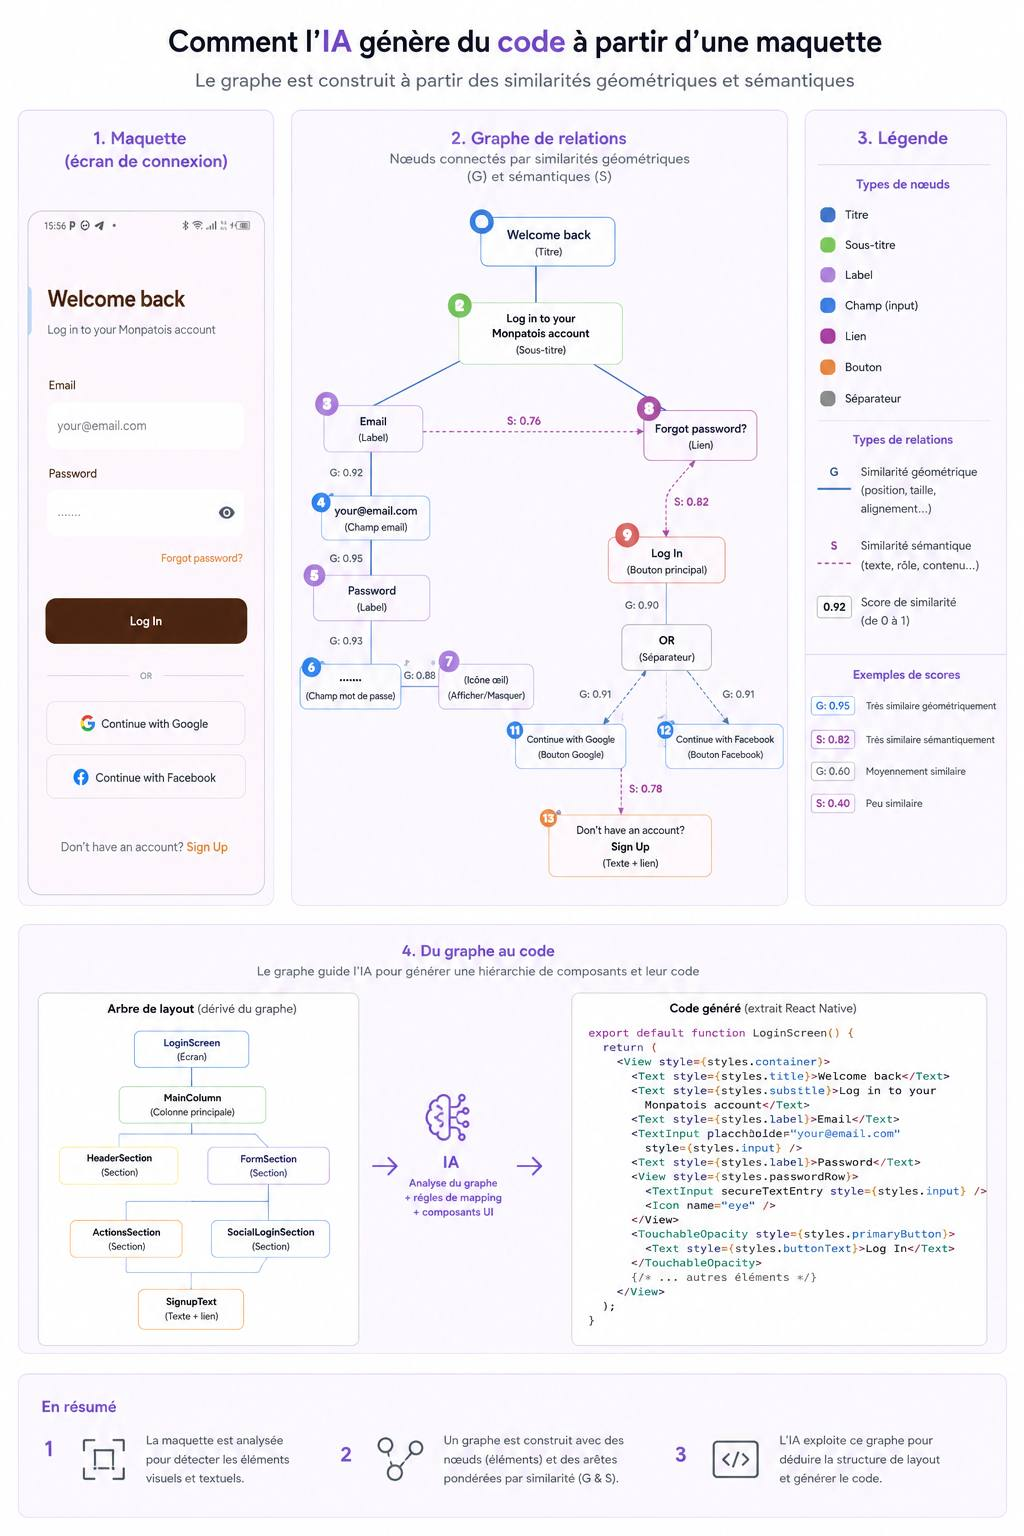
\includegraphics[height=0.82\textheight]{graph_clean.jpg}
\end{frame}

\begin{frame}{Étape 4 --- Les groupes reportés sur notre maquette}
\centering
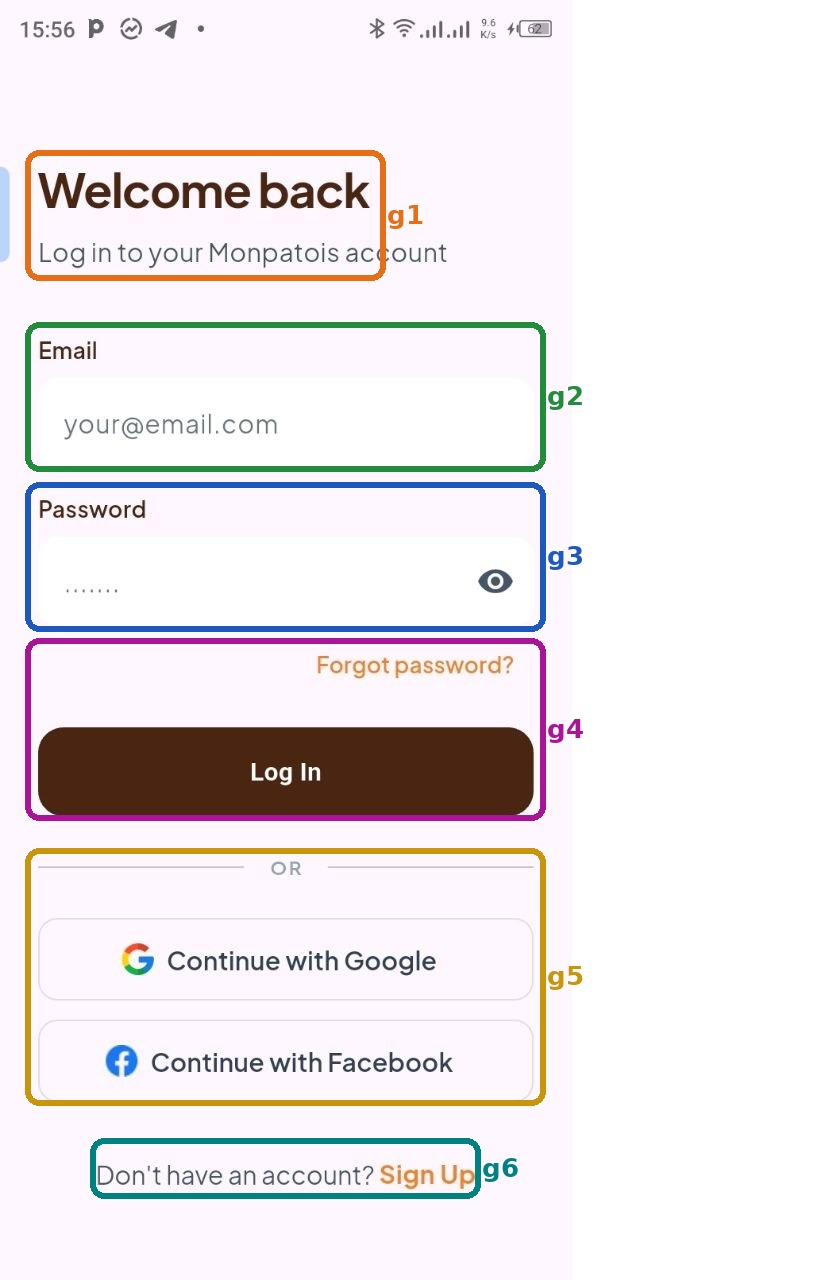
\includegraphics[height=0.85\textheight]{maquette_groups.jpg}
\end{frame}

\begin{frame}{Étape 4 --- Des groupes vers le modèle}
\begin{block}{Ce qu'on obtient}
Le graphe s'est transformé en \textbf{6 groupes logiques}, directement visibles sur notre maquette :
\end{block}
\small
\begin{itemize}
    \item $g_1$ = \{Welcome back, sous-titre\} --- en-tête
    \item $g_2$ = \{Email, champ email\} --- champ formulaire
    \item $g_3$ = \{Password, champ password\} --- champ formulaire
    \item $g_4$ = \{Forgot password?, Log In\} --- actions
    \item $g_5$ = \{OR, Google, Facebook\} --- connexion sociale
    \item $g_6$ = \{Sign Up\} --- pied de page
\end{itemize}
\end{frame}

% ============================================================
\section{Le lien entre maquette et modèle}
% ============================================================

\begin{frame}{L'idée centrale}
\begin{block}{En une phrase}
On transforme notre maquette (image, données visuelles) en modèle (graphe puis arbre, données structurelles) afin de regrouper logiquement les éléments avant de générer du code.
\end{block}

\vspace{0.3cm}
La transformation n'ajoute pas d'information nouvelle : elle rend explicite une structure qui existait déjà implicitement dans notre écran de connexion.

\vspace{0.3cm}
\begin{block}{Formulation simple}
La maquette montre \emph{ce qui est affiché}.\\
Le modèle explique \emph{comment c'est organisé}.
\end{block}
\end{frame}

\begin{frame}{Comment les deux collaborent}
\small
\begin{tabularx}{\textwidth}{@{}lXX@{}}
\toprule
\textbf{Étape} & \textbf{Rôle de la maquette} & \textbf{Rôle du modèle} \\
\midrule
Avant transformation & Fournit les éléments bruts (pixels, positions, couleurs) & N'existe pas encore \\
\addlinespace
Pendant la transformation & Sert de référence pour extraire les mesures & Se construit progressivement (graphe, groupes, arbre) \\
\addlinespace
Après transformation & Reste disponible comme vérité visuelle de contrôle & Guide la génération de code \\
\bottomrule
\end{tabularx}
\end{frame}

\begin{frame}{Références}
\footnotesize
Cette note de synthèse s'appuie sur les travaux suivants sur la reconstruction de structure à partir d'images d'interfaces :

\vspace{0.3cm}
\begin{itemize}
    \item T.~A. Nguyen et C.~Csallner. \emph{Reverse Engineering Mobile Application User Interfaces with REMAUI}. ASE 2015, p.~248--259.
    \item C.~Chen, T.~Su, G.~Meng, Z.~Xing et Y.~Liu. \emph{From UI Design Image to GUI Skeleton: A Neural Machine Translator to Bootstrap Mobile GUI Implementation}. ICSE 2018, p.~665--676.
    \item M.~Xie, Z.~Xing, S.~Feng, X.~Xu, L.~Zhu et C.~Chen. \emph{Psychologically-Inspired, Unsupervised Inference of Perceptual Groups of GUI Widgets from GUI Images}. ESEC/FSE 2022.
    \item T.~Beltramelli. \emph{pix2code: Generating Code from a Graphical User Interface Screenshot}. ACM SIGCHI EICS 2018.
\end{itemize}

\vspace{0.3cm}
\normalsize
Ces travaux formalisent, chacun à leur façon, l'idée centrale de cette présentation : détecter des éléments d'interface par proximité et par similarité visuelle, puis les regrouper en une structure exploitable pour la génération de code.
\end{frame}

\begin{frame}
\centering
{\Large\color{navy}\textbf{Merci}}
\end{frame}

\end{document}
